\documentclass[tikz,border=8pt]{standalone}
\usepackage[T1]{fontenc}
\usepackage{lmodern}
\usepackage{tikz}
\usetikzlibrary{arrows.meta,calc,positioning}

\definecolor{ink}{HTML}{172033}
\definecolor{muted}{HTML}{61708A}
\definecolor{grid}{HTML}{D9E0EA}
\definecolor{panel}{HTML}{F7F9FC}
\definecolor{stagezero}{HTML}{2F80ED}
\definecolor{stagezerofill}{HTML}{EAF3FF}
\definecolor{stageone}{HTML}{E79A19}
\definecolor{stageonefill}{HTML}{FFF4DD}
\definecolor{fullbar}{HTML}{8E5CC7}
\definecolor{emptybar}{HTML}{168B6A}

\begin{document}
\sffamily
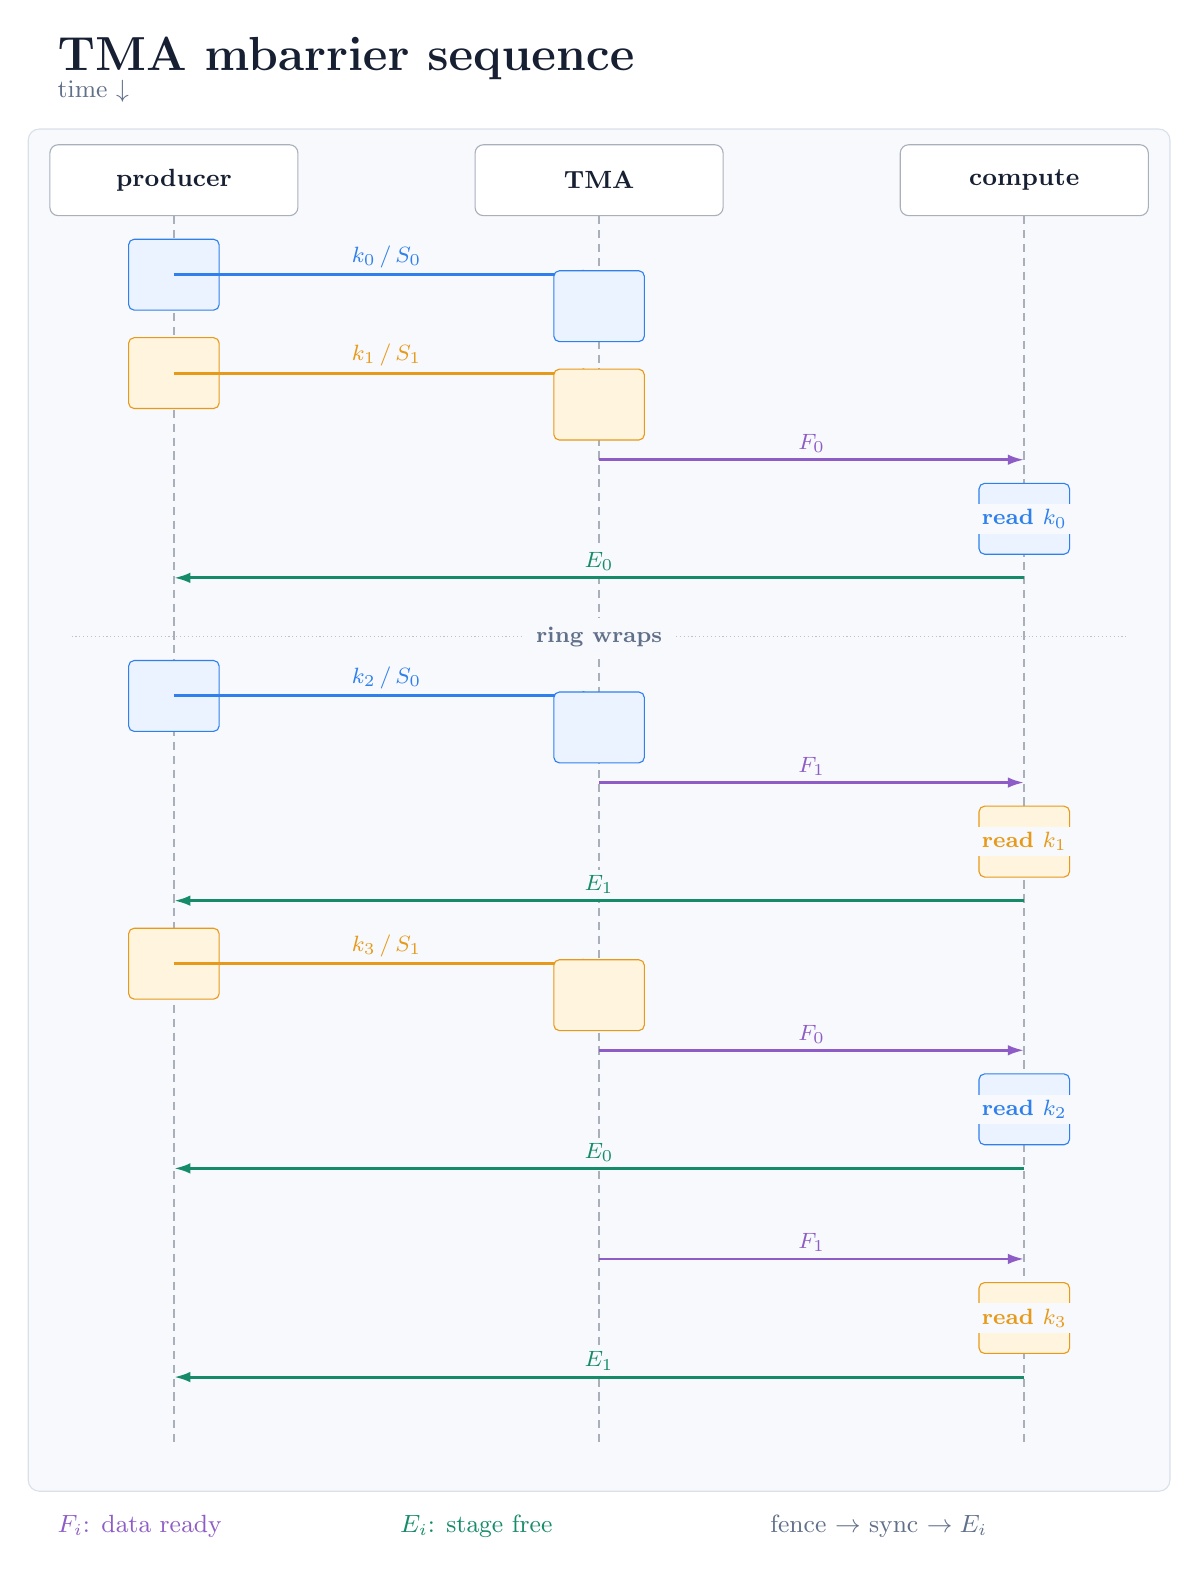
\begin{tikzpicture}[
  x=1cm,
  y=1cm,
  >={Latex[length=2.1mm,width=1.35mm]},
  title/.style={font=\bfseries\fontsize{17}{20}\selectfont, text=ink},
  subtitle/.style={font=\fontsize{9}{11}\selectfont, text=muted},
  actor/.style={draw=grid!75!ink, fill=white, rounded corners=3pt,
                minimum width=3.15cm, minimum height=9mm,
                font=\bfseries\fontsize{9}{11}\selectfont, text=ink},
  lifeline/.style={densely dashed, line width=.65pt, color=grid!75!ink},
  issue0/.style={->, line width=1.1pt, color=stagezero},
  issue1/.style={->, line width=1.1pt, color=stageone},
  full/.style={->, line width=1.05pt, color=fullbar},
  empty/.style={->, line width=1.05pt, color=emptybar},
  msg/.style={font=\bfseries\fontsize{8}{9.5}\selectfont, fill=panel, inner sep=2pt},
  action0/.style={draw=stagezero, fill=stagezerofill, rounded corners=2pt,
                  minimum width=1.15cm, minimum height=9mm},
  action1/.style={draw=stageone, fill=stageonefill, rounded corners=2pt,
                  minimum width=1.15cm, minimum height=9mm},
  actionn/.style={draw=grid!75!ink, fill=white, rounded corners=2pt,
                  minimum width=1.15cm, minimum height=7mm},
  phase/.style={font=\bfseries\fontsize{8}{10}\selectfont, text=muted,
                fill=panel, inner xsep=5pt},
]

\node[title, anchor=west] at (0,1.1) {TMA mbarrier sequence};
\node[subtitle, anchor=west] at (0,0.68) {time $\downarrow$};

\fill[panel, rounded corners=4pt] (-0.25,0.2) rectangle (14.25,-17.1);
\draw[grid, rounded corners=4pt] (-0.25,0.2) rectangle (14.25,-17.1);

\node[actor] (producer) at (1.6,-0.45) {producer};
\node[actor] (tma) at (7,-0.45) {TMA};
\node[actor] (consumer) at (12.4,-0.45) {compute};

\draw[lifeline] (producer.south) -- (1.6,-16.5);
\draw[lifeline] (tma.south) -- (7,-16.5);
\draw[lifeline] (consumer.south) -- (12.4,-16.5);

% Prologue and first refill: S1 is issued before S0 is consumed.
\node[action0] at (1.6,-1.65) {};
\draw[issue0] (1.6,-1.65) -- node[msg, text=stagezero, above] {$k_0\,/\,S_0$} (7,-1.65);
\node[action0] at (7,-2.05) {};

\node[action1] at (1.6,-2.9) {};
\draw[issue1] (1.6,-2.9) -- node[msg, text=stageone, above] {$k_1\,/\,S_1$} (7,-2.9);
\node[action1] at (7,-3.3) {};

\draw[full] (7,-4.0) -- node[msg, text=fullbar, above] {$F_0$} (12.4,-4.0);
\node[action0] at (12.4,-4.75) {};
\node[msg, text=stagezero] at (12.4,-4.75) {read $k_0$};
\draw[empty] (12.4,-5.5) -- node[msg, text=emptybar, above] {$E_0$} (1.6,-5.5);

% Reuse S0 only after E0; producer phase wraps here.
\draw[grid!85!ink, densely dotted] (0.3,-6.25) -- (13.7,-6.25);
\node[phase] at (7,-6.25) {ring wraps};
\node[action0] at (1.6,-7.0) {};
\draw[issue0] (1.6,-7.0) -- node[msg, text=stagezero, above] {$k_2\,/\,S_0$} (7,-7.0);
\node[action0] at (7,-7.4) {};

\draw[full] (7,-8.1) -- node[msg, text=fullbar, above] {$F_1$} (12.4,-8.1);
\node[action1] at (12.4,-8.85) {};
\node[msg, text=stageone] at (12.4,-8.85) {read $k_1$};
\draw[empty] (12.4,-9.6) -- node[msg, text=emptybar, above] {$E_1$} (1.6,-9.6);

\node[action1] at (1.6,-10.4) {};
\draw[issue1] (1.6,-10.4) -- node[msg, text=stageone, above] {$k_3\,/\,S_1$} (7,-10.4);
\node[action1] at (7,-10.8) {};

\draw[full] (7,-11.5) -- node[msg, text=fullbar, above] {$F_0$} (12.4,-11.5);
\node[action0] at (12.4,-12.25) {};
\node[msg, text=stagezero] at (12.4,-12.25) {read $k_2$};
\draw[empty] (12.4,-13.0) -- node[msg, text=emptybar, above] {$E_0$} (1.6,-13.0);

\draw[full] (7,-14.15) -- node[msg, text=fullbar, above] {$F_1$} (12.4,-14.15);
\node[action1] at (12.4,-14.9) {};
\node[msg, text=stageone] at (12.4,-14.9) {read $k_3$};
\draw[empty] (12.4,-15.65) -- node[msg, text=emptybar, above] {$E_1$} (1.6,-15.65);

\node[subtitle, anchor=west, text=fullbar] at (0,-17.55) {$F_i$: data ready};
\node[subtitle, anchor=west, text=emptybar] at (4.35,-17.55) {$E_i$: stage free};
\node[subtitle, anchor=west] at (9.05,-17.55) {fence $\to$ sync $\to E_i$};

\end{tikzpicture}
\end{document}
